\documentclass[12pt]{article}

\usepackage[utf8]{inputenc}
\usepackage{listings}
\usepackage{graphicx}
\usepackage{float}
\usepackage{geometry}

\usepackage{parskip}
\setlength{\parskip}{1.0\baselineskip plus2pt minus2pt}

\addtolength{\topmargin}{-50pt}
\addtolength{\textheight}{130pt}
\addtolength{\textwidth}{95pt}
\addtolength{\oddsidemargin}{-45pt}

\title{Entropia, Redundância e Informação Mútua}
\author{David Gomes, Guilherme Graça, Miguel Duarte}
\date{Outubro 2014}

\begin{document}
\maketitle
  As funções \texttt{hist} e \texttt{createHist} do primeiro exercício, embora bastante
  simples acabam por ser importantes para a visualização de dados ao longo
  de todo o projeto. Assim sendo, segue a análise ao código das mesmas.

  A função \texttt{hist} devolve a matriz \texttt{count} que contém as ocorrências
  de cada símbolo do alfabeto \texttt{A} na fonte de informação \texttt{P}. Assim,
  esta função é chamada pela função \texttt{createHist} de forma a apresentar um histograma
  com recurso à função \texttt{bar} do Matlab:

  \vspace{2mm}
  \begin{lstlisting}[language=Matlab]
  function count = createHist(P, A)
    count = hist(P, A);

    waitfor(bar(count));
  end
  \end{lstlisting}

  No ficheiro \texttt{entropia.m} encontra-se a função que calcula a entropia de acordo
  com o exercício 2 do trabalho prático. A fórmula da entropia é a seguinte:

  $$
    H(X) = \sum_{i=1}^{n}{-P(X_i) \times log_2 P(X_i)}
  $$

  No terceiro exercício recorremos às funções previamente definidas para determinar
  a entropia e a distribuição estatística em diferentes fontes de informação.
  Comecemos por observar as diferentes distribuições estatísticas.

  \begin{figure}[H]
    \centering
      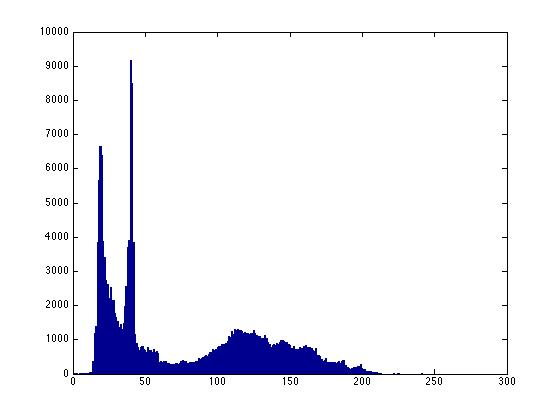
\includegraphics[width=0.75\textwidth]{ex3kid}
    \caption{Distribuição Estatística de kid.bmp}
  \end{figure}

  \begin{figure}[H]
    \centering
      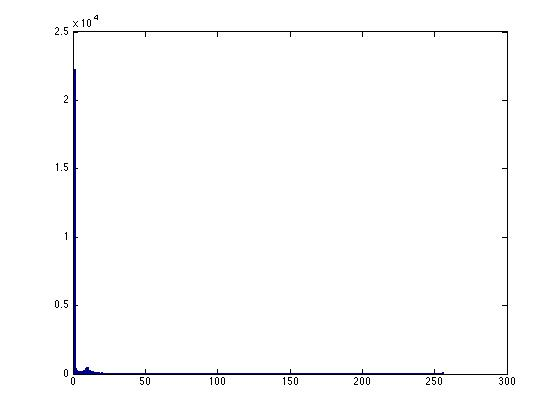
\includegraphics[width=0.75\textwidth]{ex3homer}
    \caption{Distribuição Estatística de homer.bmp}
  \end{figure}

  \begin{figure}[H]
    \centering
      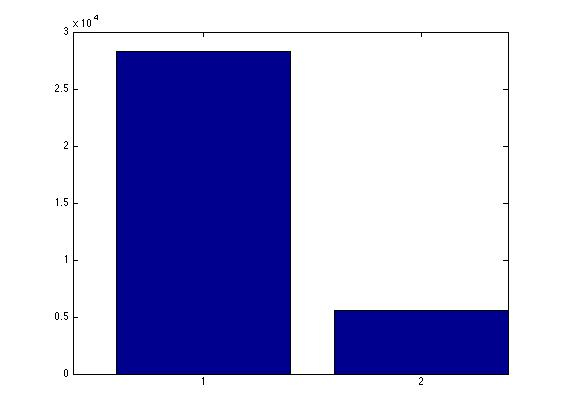
\includegraphics[width=0.75\textwidth]{ex3homerbin}
    \caption{Distribuição Estatística de homerBin.bmp}
  \end{figure}

  \begin{figure}[H]
    \centering
      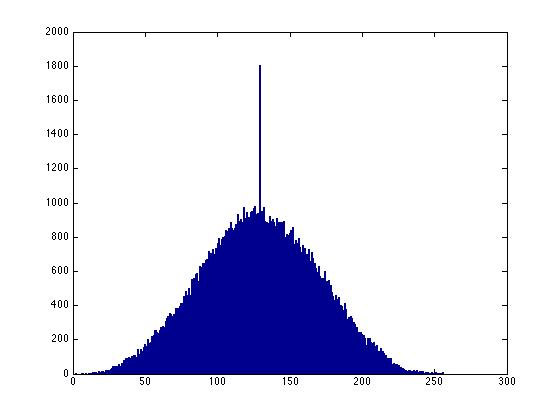
\includegraphics[width=0.75\textwidth]{ex3guitarsolo}
    \caption{Distribuição Estatística de guitarSolo.wav}
  \end{figure}

  \begin{figure}[H]
    \centering
      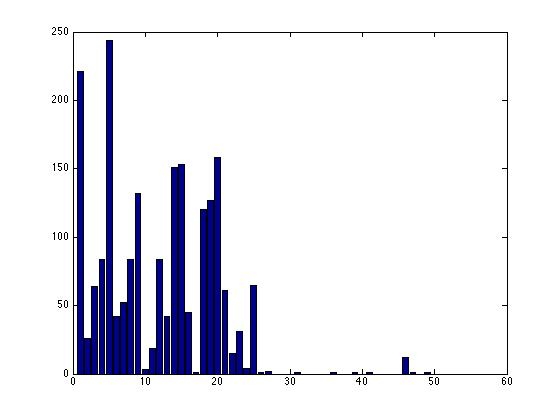
\includegraphics[width=0.75\textwidth]{ex3english}
    \caption{Distribuição Estatística de english.txt}
  \end{figure}

  Diferentes fontes de informação implicam diferentes alfabetos. Assim, usamos
  \texttt{0:255} no \texttt{kid.bmp} e no \texttt{homer.bmp}. No \texttt{homerBin.bmp},
  usamos \texttt{[0 255]} visto que as únicas duas cores presentes na imagem
  são o branco e o preto. No caso do \texttt{guitarSolo.wav}, calculamos o alfabeto
  \texttt{alf} da seguinte maneira:

  \vspace{2mm}
  \begin{lstlisting}[language=Matlab]
    quant = 7;
    d = 1 / (2^quant);
    alf = -1:d:1;
  \end{lstlisting}

  Finalmente, o alfabeto usado na fonte \texttt{english.txt} é simplesmente
  \texttt{['a':'z' 'A':'Z']}. Na figura 5, a primeira metade (\texttt{0:26})
  refere-se às letras mínusculas (\texttt{'a':'z'}), daí a maior densidade.

  Em relação a estas fontes, é colocada a questão - \textit{Sera possível
  comprimir cada uma das fontes de forma não destrutiva?}. Por um lado, a entropia
  está definida como o limite mínimo teórico blah blah blah .... Por outro lado, ...

  % WTF NAO SEI

  Apresentamos agora os valores de entropia, ou seja, o número médio mínimo
  de bits para representar cada símbolo de um dado alfabeto associado a uma
  dada fonte de informação:

  \begin{tabular}{ l c r }
    kid.bmp & 6.9541 \\
    homer.bmp & 3.4659 \\
    homerBin.bmp & 0.6448 \\
    guitarSolo.wav & 7.3580 \\
    english.txt & 4.1943 \\
  \end{tabular}

  \pagebreak

  No exercício 4, calculamos o número médio de bits por codificação
  \textit{Huffman}:

  \begin{tabular}{ l c r }
    kid.bmp & 6.9832 \\
    homer.bmp & 3.5483 \\
    homerBin.bmp & 1 \\
    guitarSolo.wav & 7.3791 \\
    english.txt & 4.2518 \\
  \end{tabular}

  Aqui coloca-se a questão - \textit{Será possível reduzir-se a variância?} -
  ao que respondemos que sim, se colocarmos os símbolos combinados na ordem
  mais elevada possível. Esta técnica é útil no caso de ...

  % WTF ^^^eu fui buscar isso a um relatorio do ano passado

  No exercício 5, calculamos o número médio de bits por símbolo (entropia)
  aplicando \textit{agrupamento de símbolos}. Por outras palavras, admitindo
  que cada símbolo é na verdade uma sequência de dois símbolos contíguos:

  \begin{tabular}{ l c r }
    kid.bmp & 4.9201 \\
    homer.bmp & 2.4198 \\
    homerBin.bmp & 0.3907 \\
    guitarSolo.wav & 5.7808 \\
    english.txt & 3.5713 \\
  \end{tabular}

  Observemos, então as distribuições estatísticas dos novos alfabetos criados
  com recurso ao agrupamento de símbolos 2 a 2:

  \begin{figure}[H]
    \centering
      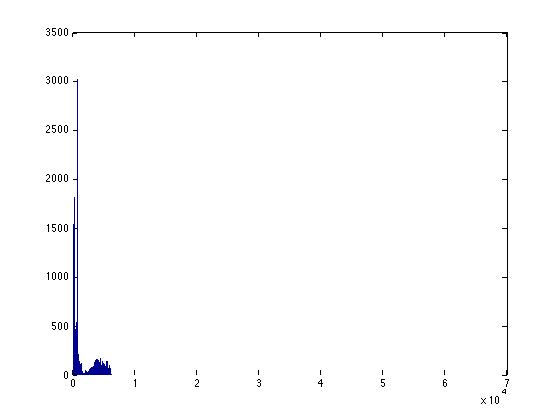
\includegraphics[width=0.75\textwidth]{ex5kid}
    \caption{Distribuição Estatística de kid.bmp}
  \end{figure}

  \begin{figure}[H]
    \centering
      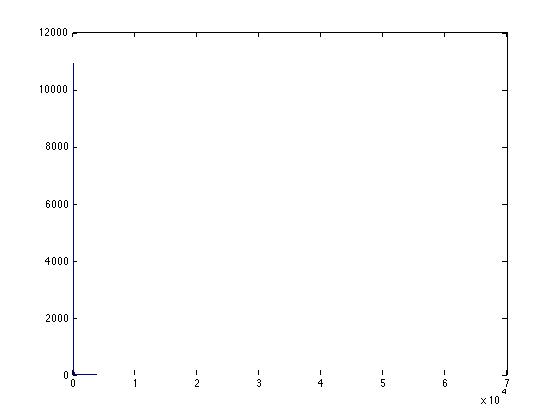
\includegraphics[width=0.75\textwidth]{ex5homer}
    \caption{Distribuição Estatística de homer.bmp}
  \end{figure}

  \begin{figure}[H]
    \centering
      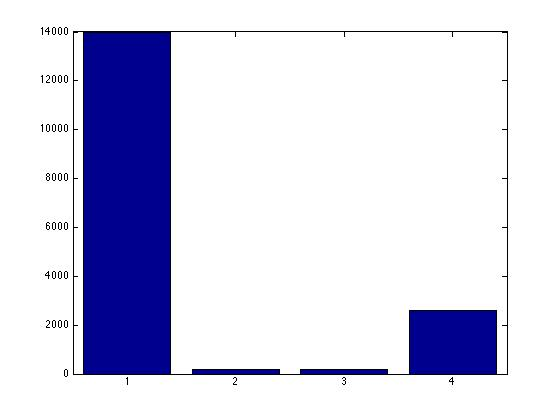
\includegraphics[width=0.75\textwidth]{ex5homerbin}
    \caption{Distribuição Estatística de homerBin.bmp}
  \end{figure}

  \begin{figure}[H]
    \centering
      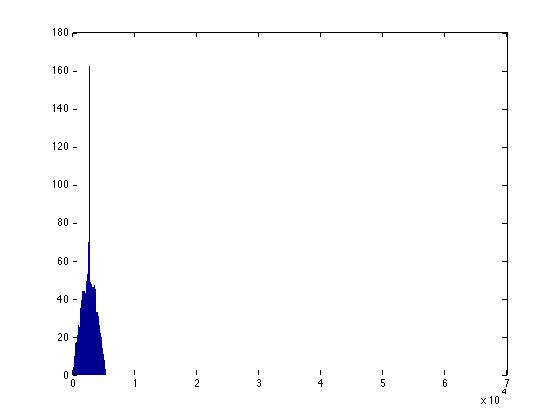
\includegraphics[width=0.75\textwidth]{ex5guitarsolo}
    \caption{Distribuição Estatística de guitarSolo.wav}
  \end{figure}

  \begin{figure}[H]
    \centering
      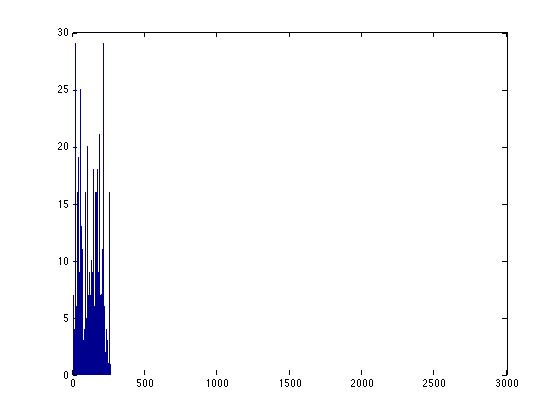
\includegraphics[width=0.75\textwidth]{ex5english}
    \caption{Distribuição Estatística de english.txt}
  \end{figure}

  De facto, o agrupamento de símbolos permite melhorar o valor
  da entropia. Isto acontece porque estudar várias variáveis em simultâneo
  é sempre preferível:

  $$ H(X ,Y) = H(X)+ H(Y|X)<= H(X)+ H(Y) $$

  O \textit{downside} está na complexidade do algoritmo e nos requisitos
  de memória que terão de ser feitos a mais.

  Finalmente, no exercício 6 vamos recorrer à informação mútua entre duas
  varíaveis de acordo com a seguinte fórmula:

  $$
    I(X,Y) = H(X) + H(Y) - H(X,Y)
  $$

  Para tal, criamos uma função chamada \texttt{slidingWindow} que
  \textit{desliza} ao longo do \texttt{target} saltando \texttt{step}
  by \texttt{step} chamando a função \texttt{mutualInf} que calcula a informação
  mútua entrea dada \texttt{query} e a atual \textit{janela} no \texttt{target}.

  Já no exercício 6.b) usamos a função \texttt{slidingWindow} para
  estudar as semelhanças entre dois ficheiros de aúdio semelhantes e
  o ficheiro \texttt{guitarSolo.wav}.

  Relembramos que no exercício 3, descobrimos que a entropia do ficheiro
  \texttt{guitarSolo.wav} é 7.3580. No \texttt{target01}
  atingimos uma entropia conjunta máxima de 7.3203 nos pontos em que
  o áudio é bastante semelhante. A melodia é igual em ambos os \textit{targets},
  daí a evolução da entropia ser igual. No entanto, no \texttt{target02},
  foi adicionado um ruído daí os valores da entropia conjunta serem
  bastante inferiores.

  \begin{figure}[H]
    \centering
    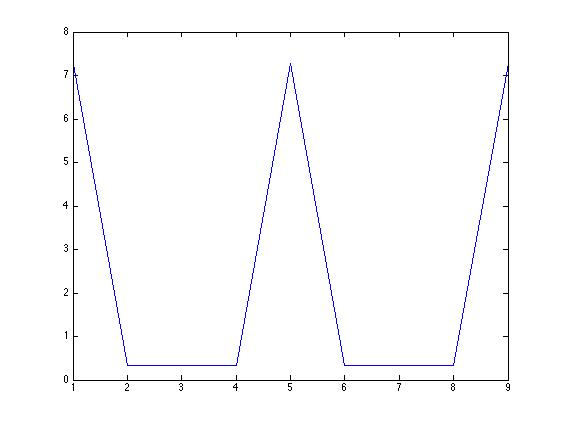
\includegraphics[width=0.5\textwidth]{ex6a}
    \caption{Evolução da entropia conjunta no target 01}
  \end{figure}

  \begin{figure}[H]
    \centering
    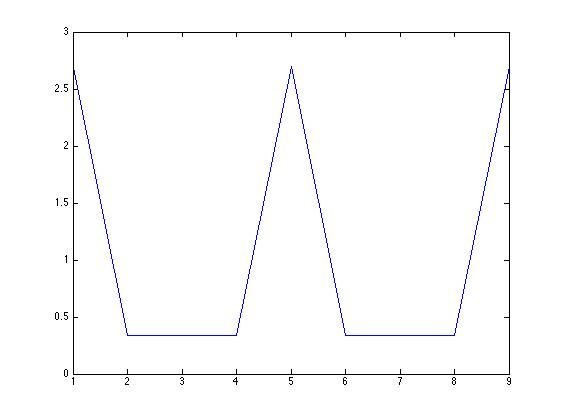
\includegraphics[width=0.5\textwidth]{ex6b}
    \caption{Evolução da entropia conjunta no target 02}
  \end{figure}

  Na última alínea, tivemos de criar uma espécie de comparador
  entre vários \textit{clips} de aúdio e o ficheiro \texttt{guitarSolo.wav}.
  O objetivo é encontrar que ficheiro tem uma parte mais semelhante com
  os ficheiro \texttt{guitarSolo.wav} e para tal fomos calcular a informação mútua
  máxima para os vários ficheiros.

  \begin{tabular}{ l c r }
    Song01.wav & 0.257843 \\
    Song02.wav & 0.377678 \\
    Song03.wav & 0.304454 \\
    Song04.wav & 0.409696 \\
    Song05.wav & 3.961751 \\
    Song06.wav & 7.338379 \\
    Song07.wav & 6.313053 \\
  \end{tabular}

  Concluímos assim que o ficheiro \texttt{Song06.wav} é o mais semelhante
  com o ficheiro \texttt{guitarSolo.wav}.
\end{document}
